%=============================================================
%  TEMPLATE PRESENTATION BEAMER - KHOA HTTT - UIT
%  Dành cho sinh viên báo cáo môn học & khóa luận
%=============================================================
\documentclass[10pt,aspectratio=169]{beamer}
\usepackage[utf8]{vietnam}
\usepackage{amsmath,amssymb,amsfonts}
\usepackage{booktabs,array,longtable}
\usepackage{graphicx}
\usepackage{tikz}
\usetikzlibrary{shapes,arrows,arrows.meta,positioning,calc,
                shapes.geometric,fit,decorations.pathreplacing,
                decorations.markings,backgrounds,shadows}
\usepackage{pgfplots}
\pgfplotsset{compat=1.18}
\usepackage[many]{tcolorbox}
\usepackage{fontawesome5}
\usepackage{hyperref}
\usepackage{listings}

%=============================================================
%  1. TEMPLATE CUSTOMIZATION (Màu sắc, Logo và Thông tin)
%  Sinh viên thay đổi các thông số dưới đây để tùy biến slide
%=============================================================
\definecolor{uitblue}{RGB}{108,79,59}       % Màu chủ đạo (Nâu đậm của header/bìa)
\definecolor{uitdark}{RGB}{74,53,37}        % Màu phụ (Nâu tối ở dải bìa/footer)
\definecolor{accent}{RGB}{197,140,50}       % Màu nhấn mạnh (Vàng Gold)
\definecolor{accentlt}{RGB}{222,178,110}    % Màu nhấn phụ (Vàng cát)
\definecolor{greenteal}{RGB}{100,120,80}    % Màu ví dụ/thực hành (Sage Green)
\definecolor{lightgray}{RGB}{248,245,240}   % Màu nền ấm của slide (Cream/Ivory)
\definecolor{textgray}{RGB}{60,55,50}       % Màu chữ thân (Charcoal)

\newcommand{\titlebgimage}{title_bg.png}
\newcommand{\sectionbgimage}{section_bg.png} % Tên tệp ảnh nền trang ngăn cách section (nếu có)     % Tên tệp ảnh nền mờ trang bìa (nếu có)
\newcommand{\logonhomNC}{logo_nhom_nc.png}   % Logo nhóm nghiên cứu/Lab (nếu có)
\newcommand{\logonhomthuchien}{logo_nhom_thuchien.png} % Logo nhóm thực hiện/CLB (nếu có)
\newcommand{\gvhd}{[Tên giảng viên hướng dẫn]}         % Giáo viên hướng dẫn (nếu có)
\newcommand{\slidewatermark}{logo_nhom_nc.png} % Tệp ảnh mờ làm hình nền từng slide (để trống nếu không dùng)
\newcommand{\contactemail}{ftisu@uit.edu.vn} % Email liên hệ hiển thị ở trang bìa

%=============================================================
%  2. THÔNG TIN BÁO CÁO (Metadata)
%=============================================================
\title[Tái hiện TiMePReSt]{Tái hiện TiMePReSt: huấn luyện DNN song song kiểu pipeline tiết kiệm thời gian và bộ nhớ}
\subtitle{Báo cáo tiến độ nghiên cứu (20/09 -- 30/09/2026)}
\author{Người thực hiện: [An Văn Kết]}
\date{Ngày báo cáo: 30/09/2026}

%=============================================================
%  3. BEAMER THEME OVERRIDE (Cấu hình hiển thị - KHÔNG NÊN SỬA)
%=============================================================
\usetheme{default}
\usecolortheme{default}
\setbeamertemplate{navigation symbols}{}

% Thiết lập màu sắc các thành phần Beamer
\setbeamercolor{palette primary}{bg=uitblue,fg=white}
\setbeamercolor{frametitle}{bg=uitblue,fg=white}
\setbeamercolor{title}{bg=uitblue,fg=white}
\setbeamercolor{author in head/foot}{bg=uitdark,fg=white}
\setbeamercolor{title in head/foot}{bg=uitblue,fg=white}
\setbeamercolor{date in head/foot}{bg=uitdark!80,fg=white}
\setbeamercolor{section in head/foot}{bg=uitblue!70,fg=white}

\setbeamercolor{block title}{bg=uitblue!18,fg=uitdark}
\setbeamercolor{block body}{bg=uitblue!5,fg=textgray}
\setbeamercolor{alertblock title}{bg=accent!20,fg=accent!80!black}
\setbeamercolor{alertblock body}{bg=accent!5,fg=textgray}
\setbeamercolor{exampleblock title}{bg=greenteal!20,fg=greenteal!70!black}
\setbeamercolor{exampleblock body}{bg=greenteal!5,fg=textgray}
\setbeamercolor{item}{fg=uitblue}
\setbeamercolor{subitem}{fg=accent}
\setbeamercolor{enumerate item}{fg=uitblue}
\setbeamercolor{normal text}{fg=textgray}
\setbeamercolor{structure}{fg=uitblue}

% Định dạng tiêu đề slide (Frametitle)
% Thiết lập hình nền mờ dưới từng slide (Watermark)
\usebackgroundtemplate{
  \ifx\slidewatermark\empty\else
    \expandafter\IfFileExists\expandafter{\slidewatermark}{
      \begin{tikzpicture}[remember picture, overlay]
        \node[opacity=0.03, anchor=center] at (current page.center) {
          \includegraphics[width=0.3\paperwidth]{\slidewatermark}
        };
      \end{tikzpicture}
    }{}
  \fi
}

\setbeamertemplate{frametitle}{
  \vskip2pt
  \begin{beamercolorbox}[wd=\paperwidth,ht=0.56cm,dp=0.2cm,leftskip=0.4cm]{frametitle}
    \usebeamerfont{frametitle}\insertframetitle
    \ifx\insertframesubtitle\empty\else
      \;{\small\textcolor{accentlt}{$\triangleright$}}\;\usebeamerfont{framesubtitle}\textcolor{accentlt}{\insertframesubtitle}
    \fi
  \end{beamercolorbox}
  \vskip-2pt
  \begin{beamercolorbox}[wd=\paperwidth,ht=1.2pt,dp=0pt]{palette primary}
    \color{accent}\rule{\paperwidth}{1.2pt}
  \end{beamercolorbox}
}

% Định dạng chân trang (Footline)
\setbeamertemplate{footline}{
  \begin{beamercolorbox}[wd=\paperwidth,ht=0.4cm,dp=0.12cm]{author in head/foot}
    \hspace{0.3cm}{\scriptsize\faUniversity\; UIT -- Khoa Hệ thống Thông tin}
    \hfill
    {\scriptsize Báo cáo khoa học}
    \hfill
    {\scriptsize\insertframenumber/\inserttotalframenumber\hspace{0.3cm}}
  \end{beamercolorbox}
}

% Định dạng đầu trang (Headline)
\setbeamertemplate{headline}{
  \begin{beamercolorbox}[wd=\paperwidth,ht=0.06cm]{section in head/foot}
    \color{accent}\rule{\paperwidth}{0.06cm}
  \end{beamercolorbox}
}

% Định dạng ký hiệu danh sách (Itemize bullets)
\setbeamertemplate{itemize item}{\color{uitblue}\faCircle[regular]}
\setbeamertemplate{itemize subitem}{\color{accent}$\triangleright$}
\setbeamertemplate{enumerate item}{\color{uitblue}\insertenumlabel.}

% Định dạng trang bìa (Title Page)
\setbeamertemplate{title page}{
  \begin{tikzpicture}[remember picture, overlay]
    \fill[uitblue] (current page.north west) rectangle ([yshift=-0.58\paperheight]current page.north east);
    \fill[uitdark] ([yshift=-0.58\paperheight]current page.north west)
         rectangle ([yshift=-0.62\paperheight]current page.north east);
    \fill[lightgray] ([yshift=-0.62\paperheight]current page.north west)
         rectangle (current page.south east);
         
    \expandafter\IfFileExists\expandafter{\titlebgimage}{
      \node[opacity=0.10, anchor=center] at (current page.center) {\includegraphics[width=\paperwidth,height=\paperheight]{\titlebgimage}};
    }{}
         
    \node[white, anchor=north west, font=\large\bfseries, align=left, text width=0.9\paperwidth] (univ) at
         ([xshift=0.5cm, yshift=-0.4cm]current page.north west)
         {\faUniversity\quad TRƯỜNG ĐẠI HỌC CÔNG NGHỆ THÔNG TIN -- UIT \\
          \small\normalfont Khoa Hệ thống Thông tin $|$ Nhóm nghiên cứu FTISU};
          
    \node[white, anchor=north west, font=\LARGE\bfseries, text width=0.88\paperwidth, align=left] (title) at
         ([yshift=-0.25cm]univ.south west)
         {\inserttitle};
         
    \node[accentlt, anchor=north west, font=\normalsize\itshape, text width=0.88\paperwidth, align=left] (subtitle) at
         ([yshift=-0.15cm]title.south west)
         {\insertsubtitle};
         
    \node[uitdark, anchor=north west, font=\small, align=left] at
         ([xshift=0.8cm, yshift=-0.66\paperheight]current page.north west)
         {\faUser\quad \insertauthor \\
          \ifx\gvhd\empty\else
            \faGraduationCap\quad GVHD: \gvhd \\
          \fi
          \faEnvelope\quad \contactemail \\
          \faCalendar\quad \insertdate};
         
    % Trang trí dòng kẻ đứng
    \draw[accent,line width=4pt]
         ([xshift=0.5cm,yshift=-0.65\paperheight]current page.north west)
      -- ([xshift=0.5cm,yshift=-0.85\paperheight]current page.north west);

    % Hiển thị Logo nhóm nghiên cứu / câu lạc bộ / khoa ở góc dưới bên phải
        % Hiển thị Logo: Nhóm NC nằm bên TRÁI nhóm thực hiện (Góc dưới bên phải)
    \expandafter\IfFileExists\expandafter{\logonhomthuchien}{
        % Vẽ Logo nhóm thực hiện trước, neo vào góc và đặt tên node là 'logo2'
        \node[anchor=south east, inner sep=0pt] (logo2) at ([xshift=-0.5cm, yshift=0.4cm]current page.south east) {
            \includegraphics[height=0.7cm]{\logonhomthuchien}
        };
        
        \expandafter\IfFileExists\expandafter{\logonhomNC}{
            % Logo nhóm NC sẽ bám vào phía bên TRÁI (west) của logo2
            \node[anchor=east, inner sep=0pt] at ([xshift=-0.2cm]logo2.west) {
                \includegraphics[height=0.7cm]{\logonhomNC}
            };
        }{}
    }{
        % Trường hợp KHÔNG có logo nhóm thực hiện, chỉ có logo nhóm NC
        \expandafter\IfFileExists\expandafter{\logonhomNC}{
            \node[anchor=south east, inner sep=0pt] at ([xshift=-0.5cm, yshift=0.4cm]current page.south east) {
                \includegraphics[height=0.7cm]{\logonhomNC}
            };
        }{}
    }
    \end{tikzpicture}
}

\AtBeginSection[]{
  {
    \usebackgroundtemplate{
      \begin{tikzpicture}[remember picture, overlay]
        \expandafter\IfFileExists\expandafter{\sectionbgimage}{
          \node[anchor=center, inner sep=0pt] at (current page.center) {
            \includegraphics[width=\paperwidth,height=\paperheight]{\sectionbgimage}
          };
        }{}
        \fill[uitblue, opacity=0.92] (current page.north west) rectangle (current page.south east);
      \end{tikzpicture}
    }
    \begin{frame}[plain]
      \centering
      \vspace{1.8cm}
      {\color{white}\Huge\bfseries\thesection}
      \par\vskip 0.3cm
      {\color{accent}\rule{0.5\paperwidth}{2pt}}
      \par\vskip 0.4cm
      {\color{accentlt}\Large\bfseries\insertsectionhead}
    \end{frame}
  }
}

%=============================================================
%  4. CÁC HỘP THÔNG TIN TCOLORBOX
%=============================================================
\tcbuselibrary{skins,breakable}

% Hộp UIT mặc định (Màu xanh chủ đạo/nâu đất)
\newtcolorbox{uitbox}[2][]{
  enhanced,
  colback=uitblue!6, colframe=uitblue, coltitle=white,
  fonttitle=\bfseries\small, title={#2},
  boxrule=0.5pt, arc=4pt, left=4pt, right=4pt, top=3pt, bottom=3pt,
  attach boxed title to top left={yshift=-2mm,xshift=4mm},
  boxed title style={colback=uitblue, arc=3pt, boxrule=0pt},
  #1
}

% Hộp Accent nhấn mạnh (Màu vàng nhấn)
\newtcolorbox{accentbox}[2][]{
  enhanced,
  colback=accent!6, colframe=accent, coltitle=white,
  fonttitle=\bfseries\small, title={#2},
  boxrule=0.5pt, arc=4pt, left=4pt, right=4pt, top=3pt, bottom=3pt,
  attach boxed title to top left={yshift=-2mm,xshift=4mm},
  boxed title style={colback=accent, arc=3pt, boxrule=0pt},
  #1
}

% Hộp ví dụ (Màu xanh lá)
\newtcolorbox{greenbox}[2][]{
  enhanced,
  colback=greenteal!6, colframe=greenteal, coltitle=white,
  fonttitle=\bfseries\small, title={#2},
  boxrule=0.5pt, arc=4pt, left=4pt, right=4pt, top=3pt, bottom=3pt,
  attach boxed title to top left={yshift=-2mm,xshift=4mm},
  boxed title style={colback=greenteal, arc=3pt, boxrule=0pt},
  #1
}

%=============================================================
%  5. CÁC MACRO RÚT GỌN (Tô màu từ khóa)
%=============================================================
\newcommand{\highlight}[1]{\textcolor{accent}{\bfseries #1}}
\newcommand{\kw}[1]{\textcolor{uitblue}{\bfseries #1}}

%=============================================================
%  PHẦN THÂN TÀI LIỆU
%=============================================================
\begin{document}
\newcolumntype{L}[1]{>{\raggedright\arraybackslash}p{#1}}

%--- Slide 1: Trang bìa ---
{
  \usebackgroundtemplate{}
  \begin{frame}[plain]
    \titlepage
  \end{frame}
}

%--- Slide 2: Bài toán và những gì đã làm ---
\begin{frame}{Bài toán và những gì đã thực hiện}
\begin{columns}[T]
\column{0.49\textwidth}
\begin{uitbox}{\faLightbulb\; TiMePReSt khác PipeDream ở hai điểm}
\footnotesize
\begin{itemize}
  \item \kw{Lịch nF1B:} forward lần lượt $N$ micro-batch rồi \textbf{một} backward chung (PipeDream: 1F1B \cite{narayanan2019pipedream}).
  \item \kw{Bỏ horizontal stashing:} backward dùng trọng số mới nhất; vẫn giữ vertical synchronization.
\end{itemize}
\end{uitbox}
\vspace{0.1cm}
\begin{accentbox}{\faBullseye\; Mục tiêu kiểm chứng}
\footnotesize
Ba kết quả chính của bài báo \cite{dutta2026timeprest}: \highlight{chất lượng} ngang PipeDream, \highlight{thời gian}/epoch ngắn hơn, \highlight{bộ nhớ} GPU thấp hơn.
\end{accentbox}

\column{0.47\textwidth}
\begin{greenbox}{\faTools\; Đã xây dựng}
\footnotesize
\begin{itemize}
  \item Cài đặt lại PipeDream và TiMePReSt trên PyTorch mới (mã nguồn bài báo không công bố).
  \item Bản mô phỏng 1 GPU và bản \textbf{pipeline thực 2 GPU} (Kaggle T4$\times$2).
  \item Lịch chạy khớp Fig.~2 của bài báo; phiên bản trọng số đúng mô tả; kiểm tra $v = 1$ khi $W \le N+1$.
\end{itemize}
\end{greenbox}
\end{columns}
\end{frame}

%--- Slide 3: Thiết lập thí nghiệm ---
\begin{frame}{Thiết lập thí nghiệm}
\begin{columns}[T]
\column{0.56\textwidth}
\begin{uitbox}{\faServer\; Hạ tầng: bài báo và thí nghiệm này}
\scriptsize
\setlength{\tabcolsep}{3pt}
\renewcommand{\arraystretch}{1.1}
\begin{tabular}{@{}L{1.6cm}L{3.0cm}L{2.3cm}@{}}
\toprule
 & \textbf{Bài báo} & \textbf{Thí nghiệm này} \\
\midrule
Máy & 2--4 máy riêng (1 GPU/máy), nối mạng & 1 máy, 2 GPU \\
GPU & Quadro RTX 6000, RTX 2080 & 2 $\times$ T4 16 GB \\
Số stage $W$ & 2, 3, 4 & 2 \\
Micro-batch & $N = 3$ & $N = 3$, mini-batch 192 \\
Siêu tham số & Không nêu & SGD, lr chọn bằng sweep \\
\bottomrule
\end{tabular}
\end{uitbox}

\column{0.40\textwidth}
\begin{greenbox}{\faFlask\; Các thí nghiệm đã chạy}
\scriptsize
\begin{itemize}
  \item \kw{VGG-16 / CIFAR-100}, 160 epoch
  \item \kw{VGG-16 / Tiny-ImageNet}, 80 epoch, 3 seed; ablation Variant 1/2, DeepSpeed, PipeDream theo micro-batch
  \item \kw{ResNet-50 / Tiny-ImageNet}, 80 epoch
  \item \kw{Giả lập mạng chậm} 0,5--10 Gbit/s giữa hai GPU
\end{itemize}
\end{greenbox}
\end{columns}
\vspace{0.1cm}
\begin{accentbox}{\faProjectDiagram\; Ablation của bài báo (\S4.10)}
\scriptsize
Mỗi variant chỉ giữ \textbf{một} trong hai thay đổi của TiMePReSt: \kw{Variant 1} = lịch nF1B + \textbf{giữ} weight stashing; \kw{Variant 2} = lịch 1F1B + \textbf{bỏ} weight stashing.
\end{accentbox}
\end{frame}

%--- Slide 4: Chất lượng ---
\begin{frame}{Kết quả: chất lượng mô hình}
\centering
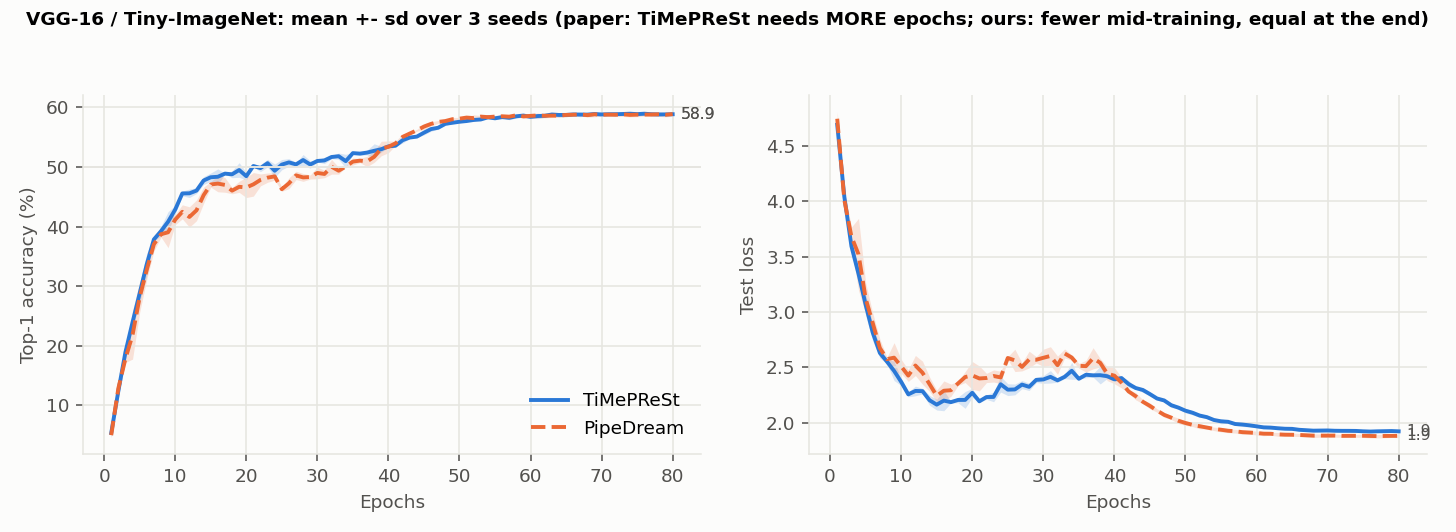
\includegraphics[width=0.72\textwidth]{images/fig08b_vgg16_tinyimagenet_3seeds.png}\\[-0.1cm]
{\tiny VGG-16 / Tiny-ImageNet, 80 epoch, trung bình $\pm$ độ lệch chuẩn qua 3 seed (tương ứng Fig.~8 của bài báo)}
\vspace{0.05cm}
\begin{columns}[T]
\column{0.48\textwidth}
\begin{greenbox}{\faCheckCircle\; Giống bài báo: chất lượng cuối ngang nhau}
\scriptsize
Top-1 TiMePReSt / PipeDream: CIFAR-100 \textbf{72,4 / 72,2\%}; Tiny-ImageNet \textbf{58,9 / 58,9\%}; ResNet-50 \textbf{66,5 / 65,4\%}.
\end{greenbox}
\column{0.48\textwidth}
\begin{accentbox}{\faExclamationTriangle\; Khác bài báo: học nhanh hơn ở giữa}
\scriptsize
Đạt 50\% top-1 sau \textbf{20 epoch} (PipeDream: \textbf{31}). Bài báo nói TiMePReSt cần \emph{nhiều} epoch hơn.
\end{accentbox}
\end{columns}
\end{frame}

%--- Slide 5: Thời gian ---
\begin{frame}{Kết quả: thời gian huấn luyện}
\centering
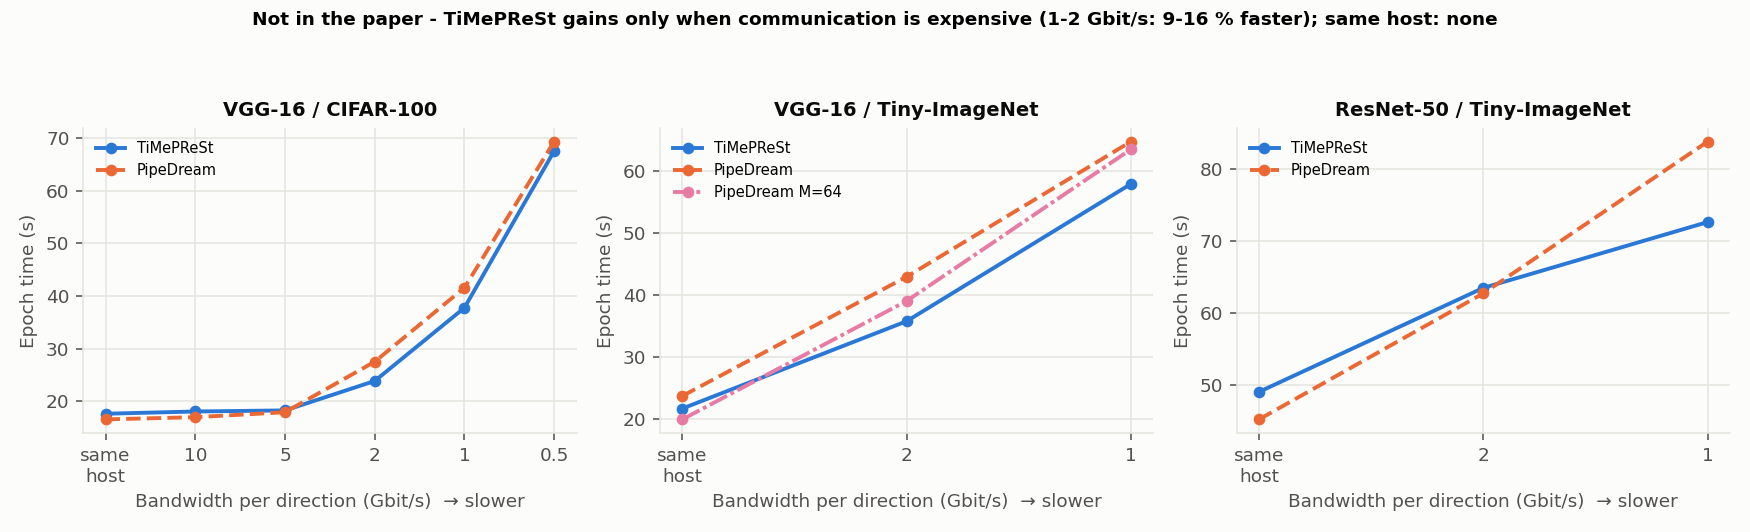
\includegraphics[width=0.84\textwidth]{images/figX_bandwidth.png}\\[-0.1cm]
{\tiny Thời gian mỗi epoch: ``same host'' = 2 GPU trên cùng một máy; các điểm còn lại = giả lập đường truyền giữa 2 GPU như hai máy nối mạng (càng sang phải mạng càng chậm)}
\vspace{0.05cm}
\begin{columns}[T]
\column{0.48\textwidth}
\begin{accentbox}{\faExclamationTriangle\; 2 GPU cùng máy: chưa có lợi thế}
\scriptsize
Hai GPU trên cùng một máy Kaggle: thời gian/epoch của PipeDream bằng \textbf{0,92--1,09 lần} TiMePReSt; bài báo: PipeDream chậm hơn \textbf{1,7--5,7 lần}.
\end{accentbox}
\column{0.48\textwidth}
\begin{greenbox}{\faCheckCircle\; 2 GPU khác máy (giả lập): có lợi thế}
\scriptsize
Giả lập hai GPU ở hai máy nối mạng 1--2 Gbit/s như bài báo: TiMePReSt nhanh hơn \textbf{9--16\%}/epoch nhờ vừa truyền vừa tính theo micro-batch.
\end{greenbox}
\end{columns}
\vspace{0.05cm}
{\tiny\textit{Mức nhanh hơn 31\% báo cáo tuần trước do baseline cũ chưa đúng PipeDream; đã cài đặt lại theo mã nguồn gốc.}}
\end{frame}

%--- Slide 6: Bộ nhớ ---
\begin{frame}{Kết quả: bộ nhớ GPU}
\centering
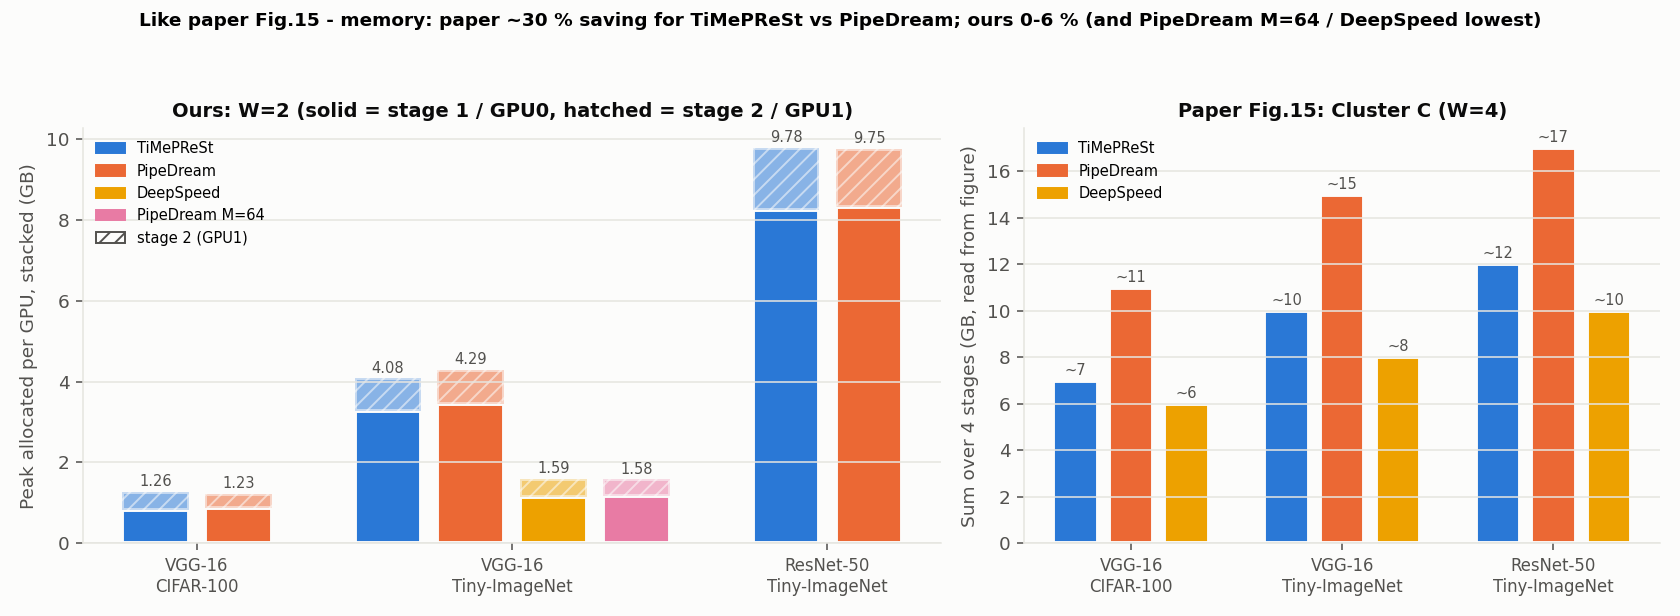
\includegraphics[width=0.76\textwidth]{images/fig15_memory.png}\\[-0.1cm]
{\tiny Bộ nhớ đỉnh mỗi GPU: thí nghiệm này (trái, $W = 2$) và Fig.~15 của bài báo (phải, $W = 4$)}
\vspace{0.05cm}
\begin{columns}[T]
\column{0.48\textwidth}
\begin{accentbox}{\faExclamationTriangle\; Chưa tái hiện: tiết kiệm $\sim$30\%}
\scriptsize
Tổng bộ nhớ hai hệ gần bằng nhau; GPU0 chỉ giảm \textbf{1--6\%}, GPU1 có trường hợp tăng.
\end{accentbox}
\column{0.48\textwidth}
\begin{uitbox}{\faSearch\; Lý do dự đoán}
\scriptsize
Có thể do chỉ có 2 stage: bỏ stashing chỉ bớt một phiên bản trọng số ở stage 1 ($\sim$5 MB), nhỏ so với activation; bài báo đo ở 4 stage.
\end{uitbox}
\end{columns}
\end{frame}

%--- Slide 7: Tổng hợp và nguyên nhân ---
\begin{frame}{Tổng hợp so với bài báo và nguyên nhân}
\begin{columns}[T]
\column{0.50\textwidth}
\begin{uitbox}{\faBalanceScale\; Đối chiếu các kết quả chính}
\scriptsize
\setlength{\tabcolsep}{3pt}
\renewcommand{\arraystretch}{1.35}
\begin{tabular}{@{}L{3.0cm}L{3.2cm}@{}}
\toprule
\textbf{Bài báo} & \textbf{Thí nghiệm này} \\
\midrule
Chất lượng ngang PipeDream & \textcolor{greenteal}{\textbf{Tái hiện được}} \\
Nhanh hơn 1,7--5,7 lần/epoch & \textcolor{accent}{\textbf{Có điều kiện:}} 9--16\% khi mạng chậm \\
Tiết kiệm bộ nhớ $\sim$30\% & \textcolor{red!60!black}{\textbf{Chưa:}} 0--6\% \\
Cần nhiều epoch hơn & \textcolor{red!60!black}{\textbf{Ngược lại}} \\
Variant 1 (nF1B, giữ stashing) tốt hơn TiMePReSt & \textcolor{red!60!black}{\textbf{Chưa:}} ngang nhau \\
DeepSpeed ít bộ nhớ hơn & \textcolor{greenteal}{\textbf{Tái hiện được}} (ít hơn 2,5--3 lần) \\
\bottomrule
\end{tabular}
\end{uitbox}

\column{0.46\textwidth}
\begin{accentbox}{\faSearch\; Nguyên nhân dự đoán}
\scriptsize
\begin{itemize}
  \item \kw{Hạ tầng:} truyền dữ liệu trong cùng máy rất rẻ nên lợi thế vừa truyền vừa tính không phát huy; 2 stage nên stashing tiết kiệm ít. Chưa giải thích được mức chênh 5--6 lần.
  \item \kw{Bài báo thiếu chi tiết:} không mô tả cách tính backward khi forward/backward dùng hai phiên bản trọng số; mô tả baseline PipeDream không nhất quán (\S4.5 và Eq.~17).
  \item \kw{Ablation:} Variant 1 (lịch nF1B nhưng vẫn giữ weight stashing) học nhanh như TiMePReSt $\Rightarrow$ lợi thế đến từ lịch nF1B, không phải từ việc bỏ stashing.
\end{itemize}
\end{accentbox}
\end{columns}
\end{frame}

%--- Slide 8: Kết luận ---
\begin{frame}{Kết luận}
\begin{uitbox}{\faFlag\; Kết luận}
\footnotesize
\begin{itemize}
  \item Trên 2 GPU cùng máy, TiMePReSt đạt \highlight{chất lượng tương đương} PipeDream.
  \item Lợi thế \highlight{thời gian} chỉ xuất hiện khi truyền dữ liệu giữa các stage tốn kém (giả lập mạng chậm); lợi thế \highlight{bộ nhớ} chưa tái hiện được.
  \item Một số kết quả chưa kiểm chứng đầy đủ do bài báo thiếu mô tả chi tiết (cách tính backward, cấu hình baseline).
\end{itemize}
\end{uitbox}
\vspace{0.15cm}
\begin{uitbox}{\faBook\; Tài liệu tham khảo}
\tiny
\bibliographystyle{apalike}
\bibliography{references}
\end{uitbox}
\end{frame}

\end{document}
